\documentclass[11pt,a4paper]{article}
\usepackage[english,greek]{babel}
\usepackage[utf8]{inputenc}
\usepackage[margin=1in]{geometry}
\usepackage{amsthm,amsmath,amssymb,caption,graphicx,extarrows,float,changepage}
\usepackage{tikz}
\usepackage[colorlinks, allcolors=black]{hyperref}

\usepackage{libertine}
\usepackage{libertinust1math}

\newcommand{\R}{{\mathbb{R}}}

\newcommand{\en}[1]{\foreignlanguage{english}{#1}}
\newcommand{\pn}[1]{\left({#1}\right)}

\let\sin\relax
\DeclareMathOperator{\sin}{\text{ημ}}

% Tikz
\tikzset{
	closed point/.style={circle, minimum width=2mm, inner sep=0pt, fill=black, draw=black},
	open point/.style={circle, minimum width=2mm, inner sep=0pt, fill=white, draw=black},
}

\title{{\Huge\bfseries Επαναληπτικό Dιαγώνισμα}\\[1ex]\Large Μέχρι και το ΘΜΤ}
\author{\href{https://aftermaths.gr}{\en{aftermaths.gr}}}
\date{\today}

\newtheoremstyle{myStyle}
{\topsep}
{\topsep}
{}
{}
{\bfseries}
{}
{\newline}
{}

\theoremstyle{myStyle}

\newtheorem{them}{Θέμα}

\begin{document}
	\maketitle
	\begin{them}[25 μονάδες]
		\begin{enumerate}
			\item Πότε λέμε ότι μία συνάρτηση $f$ είναι παραγωγίσιμη σε ένα κλειστό διάστημα $[\alpha,\beta]$? (3 μονάδες)
			\item Να διατυπώσετε το Θεώρημα το \en{Rolle} και να δώσετε τη γεωμετρική του ερμηνεία. (7 μονάδες)
			\item Να αποδείξετε ότι αν μία συνάρτηση $f$ είναι παραγωγίσιμη σε ένα σημείο $x_0$ του πεδίου ορισμού της τότε είναι και συνεχής σε αυτό. (5 μονάδες)
			\item Να χαρακτηρίσετε τις παρακάτω προτάσεις ως \textit{Σωστές} ή \textit{Λανθασμένες} (χωρίς αιτιολόγηση) σημειώνοντας στο 
			χαρτί σας τον αριθμό της πρόταση και δίπλα την λέξη \textbf{Σωστό} ή \textbf{Λάθος}, αντίστοιχα (10 μονάδες):
			\begin{enumerate}
				\item Αν μία συνάρτηση $f$ ικανοποιεί τις υποθέσεις του Θεωρήματος Μέσης Τιμής σε ένα κλειστό διάστημα $[\alpha,\beta]$ τότε ικανοποιεί και τις υποθέσεις του Θεωρήματος \en{Rolle} σε αυτό το διάστημα.
				\item $(\ln3)'=\frac{1}{3}$.
				\item Η εξίσωση $x^3+\ln(e^x+1)=0$ έχει μοναδική λύση στο $\R$.
				\item Κάθε πολυώνυμο περιττού βαθμού έχει τουλάχιστον μία πραγματική ρίζα.
				\item Αν μία παραγωγίσιμη συνάρτηση $f:\R\to(0,+\infty)$ ικανοποιεί τη σχέση $f^2(x)\geq f^2(4)$ τότε $f'(4)=0$.
			\end{enumerate}
		\end{enumerate}
	\end{them}

	\begin{them}[25 μονάδες]
		Δίνεται η συνάρτηση $f:\R\to\R$ με τύπο:
		\[f(x)=x^2+\ln(x^2+4),\quad x\in\R.\]
		\begin{enumerate}
			\item Να μελετήσετε την $f$ ως προς την μονοτονία και τα ακρότατα. (7 μονάδες)
			\item Να βρείτε το πλήθος των ριζών της εξίσωσης $f(x)=\lambda$ για τις διάφορες τιμές του $\lambda\in\R$. (5 μονάδες)
			\item Να αποδείξετε ότι υπάρχουν μοναδικά $\xi_1,\xi_2\in\R$ με $\xi_1\xi_2<0$ που να ικανοποιούν τη σχέση $f(x)=2-x$. (6 μονάδες)
			\item Να αποδείξετε ότι για κάθε $x\in\R$ ισχύει ότι: (7 μονάδες)
			\[4x^2+1\geq4x+\ln\frac{4}{4x^2-4x+5}.\]
		\end{enumerate}
	\end{them}
	
	\begin{them}[25 μονάδες]
		\begin{minipage}{0.48\textwidth}
			Δίνεται μία συνεχής συνάρτηση $f:[-2,4]\to\R$ η οποία είναι παραγωγίσιμη στο $(-2,4)$ και η παράγωγός της, $f'$, έχει τη γραφική παράσταση που φαίνεται στο Σχήμα~\ref{fig:derivative}. Επίσης, ισχύει ότι:
			\[\lim_{x\to2}\pn{f^2(x)+6f(x)}=9.\]
			\begin{enumerate}
				\item Να δείξετε ότι $f(2)=-3$. (3 μονάδες)
				\item Να βρείτε την εξίσωση της εφαπτομένης της γραφικής παράστασης της $f$ στο $A(2,f(2))$. (3 μονάδες)
				\item Να δείξετε ότι $f(x)<f'(x)+f(x-1)$ για κάθε $x\in(0,4)$. (5 μονάδες)
				\item Να δείξετε ότι $f([-2,4])\subseteq(-19,5)$. (7 μονάδες).
				\item Να δείξετε ότι η παρακάτω εξίσωση έχει το πολύ τρεις ρίζες στο $[-2,4]$ (7 μονάδες):
				\[e^{f^2(x)}-e^{6f(x)}=e^{6f(x)}\pn{6f(x)-f^2(x)}\]
			\end{enumerate}
		\end{minipage}
		\hfill%
		\begin{minipage}{0.5\textwidth}
			\centering
			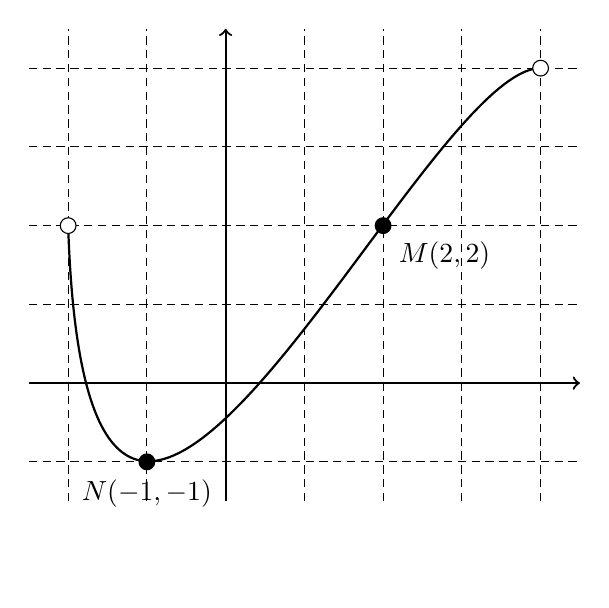
\begin{tikzpicture}
				\draw[thick, ->] (-2.5,0) -- (4.5,0);
				\draw[thick, ->] (0,-1.5) -- (0,4.5);
				\draw[densely dashed, thin] (-2.5,-1.5) grid (4.5,4.5);
				\begin{scope}
					\clip (-2.5,-2.5) rectangle (4.5,4.5);
					\draw[thick] (-2,2) .. controls (-1.75,-5.75) and (2.45,4) .. (4,4);
				\end{scope}
				\node[open point] (a) at (-2,2) {};
				\node[open point] (b) at (4,4) {};
				\node[closed point, label={315}:{$M(2,2)$}] (m) at (2,2) {};
				\node[closed point, label={270}:{$N(-1,-1)$}] (n) at (-1,-1) {};
			\end{tikzpicture}
			\captionof{figure}{Η γραφική παράσταση της $f'$}
			\label{fig:derivative}
		\end{minipage}
	\end{them}
	
	\begin{them}[25 μονάδες]
		Δίνεται μία συνάρτηση $f:(0,\pi)\to\R$ που ικανοποιεί τη σχέση:
		\[e^{f(x)}-xe^{\sin x}=\sin x+\ln x-f(x),\quad x\in(0,\pi).\]
		\begin{enumerate}
			\item Να δείξετε ότι $f(x)=\sin x+\ln x$, $x\in(0,\pi)$. (5 μονάδες)
			\item Να δείξετε ότι η $f'$ έχει μοναδική ρίζα $\rho\in(0,\pi)$. (5 μονάδες)
			\item Να δείξετε ότι για κάθε $x\in(0,\pi)$ (7 μονάδες):
			\[f(x)+\ln2\leq \frac{2x}{\pi}+\ln\pi.\]
			\item Να δείξετε ότι η $f$ έχει μοναδική ρίζα $\xi\in(0,\pi)$. (8 μονάδες)
		\end{enumerate}
	\end{them}
	\vfill
	\centering
	\textbf{Καλή Επιτυχία!}
\end{document}